\subsubsection{Filtro de Kalman}

El filtro de Kalman es un algoritmo de estimación utilizado para predecir el estado de un sistema dinámico mediante la combinación de datos provenientes de uno o mas sensores, considerando la incertidumbre y el ruido de medición. En el contexto del robot omnidireccional del presente proyecto, este filtro tiene un rol crucial, ya que permite corregir errores en la localización, estimar velocidades más precisas y mejorar la trayectoria mediante la integración de señales provenientes de múltiples sensores.

El funcionamiento del filtro de Kalman se basa en dos etapas: la predicción, donde se estima el próximo estado del sistema utilizando el modelo matemático exacto o teórico; y la actualización, en la que se corrige esa estimación en función de las mediciones actuales, aplicando un modelo probabilístico para minimizar el error. Mediante su modelo probabilístico, es capaz de filtrar el ruido y las imprecisiones de las mediciones, lo que permite obtener una representación confiable del estado.

En cuanto a su implementación, se desarrollará una integración entre el modelo cinemático existente y el filtro de Kalman en Python. Los resultados esperados incluyen un aumento significativo en la precisión de la navegación del robot y una mejora en su capacidad de adaptarse a entornos ruidosos.


\paragraph{Estimación del estado} \mbox{} \vspace{10pt}

A través de un modelo probabilístico, el filtro combina las predicciones del sistema basadas en el modelo cinemático con mediciones reales provenientes de sensores. Esto permite minimizar el impacto del ruido y las imprecisiones inherentes a las lecturas de los sensores. El proceso de estimación sigue dos etapas principales:

\begin{itemize}
    \item Predicción: Utilizando el modelo de movimiento del robot, se genera una estimación inicial del estado en el instante de tiempo dado.
    \item Actualización: Esta estimación se corrige comparándola con las mediciones obtenidas en tiempo real, ajustando los valores según la incertidumbre de cada fuente de datos. El resultado es una representación más precisa del estado actual del robot.
\end{itemize}

La información estimada por el filtro de Kalman se utiliza para compensar trayectorias y corregir vectores de movimiento. En caso de detectar desviaciones respecto a la trayectoria deseada, se ajustan dinámicamente los comandos de control (distancia y velocidad) enviados al robot, compensando errores como ser resbalamiento, impactos externos e irregularidades del terreno. Esto asegura que el robot mantenga su rumbo previsto con alta precisión y adaptabilidad a entornos variables, además, la capacidad de compensación mejora la fluidez de los desplazamientos.

En términos prácticos, la implementación del filtro de Kalman no solo refuerza la fiabilidad del sistema de navegación, sino que también sienta una base sólida para futuros desarrollos, como la integración con sensores más avanzados o la aplicación en sistemas autónomos.


\paragraph{Matrices de covarianza} \mbox{} \vspace{10pt}

Las matrices de covarianza expresan la relación estadística entre las distintas variables del sistema, cuantificando tanto la magnitud del ruido como la correlación entre las mediciones obtenidas de diferentes sensores. Cada elemento de la matriz de covarianza representa cómo dos variables están relacionadas en términos de su varianza compartida; por lo tanto, si las variables son independientes, sus valores excepto los de la diagonal principal de la matriz son nulos.

El propósito de estas matrices en el filtro de Kalman y en sistemas similares radica en su capacidad para modelar la incertidumbre. Se utilizan tanto en la etapa de predicción, como en la de actualización del filtro para ponderar el impacto de los errores de medición, mejorando las estimaciones del estado. \cite{tzafestas2013introduction} \cite{Rigatos01062007}

La calibración de las matrices de covarianza es crucial para garantizar su correcta representación del ruido real del sistema. Esto puede lograrse mediante técnicas experimentales, analizando mediciones históricas para calcular las varianzas y covarianzas directamente. También se pueden implementar métodos estadísticos que ajusten las matrices iterativamente según los resultados obtenidos durante el funcionamiento del robot. Otra técnica consiste en realizar simulaciones repetitivas, diseñadas para identificar los patrones de error y ajustar las matrices en consecuencia. \cite{Bang18}

\paragraph{Cambio de coordenadas medición/estimación} \mbox{} \vspace{10pt}

Dado que en la próxima iteración se va a colocar una cámara fija en el robot que queremos que esté siempre apuntando hacia el frente, cuando el robot realiza trayectorias y necesita hacer un cambio de dirección, primero realiza un giro sobre su propio eje hasta orientar al robot correctamente.

Por otro lado, el robot al moverse siempre a lo largo sobre su propio eje $y$, va a reportar siempre mediciones donde la velocidad $v_y$ es distinta de cero y $v_x$ es cercana a cero. Es por ello que se agrega una variable que lleva la cuenta de la orientación del robot en grados $[0^{\circ}, 90^{\circ}, 180^{\circ}, 270^{\circ}]$ respecto al sistema de coordenadas global. Con esta información realizamos un cambio de coordenadas para adaptar el sistema de coordenadas locales del robot y sus mediciones, a las globales del mapa.

\paragraph{Implementación} \mbox{} \vspace{10pt}

El filtro de Kalman se implementa de modo que registra velocidad y posición en un eje determinado, por lo que replicando el filtro 2 veces podemos tener una representación de un plano $XY$. Esta implementación se realiza en Python y se integra al funcionamiento del sistema.

Del filtro de Kalman 2D registramos la siguiente tupla:
$$ [x, v_x, y, v_y] $$

Siendo $x$ la posición absoluta en el eje $x$, $v_x$ la velocidad en el eje $x$, $y$ la posición absoluta en el eje $y$ y $v_y$ la velocidad en el eje $y$. Cada Filtro de Kalman se encarga de cada eje $X$ e $Y$ en particular.
Es importante que la entrada y salida del filtro sean del mismo formato, es decir, tenga como entrada y salida la tupla $[x, v_x, y, v_y]$. En este caso introducimos las mediciones acumuladas en distancia y las velocidades en cada eje cartesiano.

La secuencia de procesos a realizar cada vez que se recibe una medición es el siguiente:
\begin{enumerate}
    \item Cálculo del Estado Predicho $X_{kp}$.
    \item Cálculo de la Matriz de Covarianza de Proceso Predicha $P_{kp}$.
    \item Cálculo de la ganancia de Kalman $K$.
    \item Cálculo del Estado Estimado $X_k$.
    \item Actualización de valores.
    \item Actualización de la Matriz de Covarianza de Proceso $P_k$.
\end{enumerate}

Por otra parte, esperamos que el funcionamiento del Filtro de Kalman sea tal que podamos actualizar el estado por cada medición recibida del robot y calcular el vector de compensación según el estado estimado por el filtro. Este proceso se describe en el diagrama de secuencia de la Figura \ref{fig:diagsecuenciafiltrokalman}. \\


\textbf{Adaptación de datos de entrada} \mbox{} \vspace{10pt}

Para comenzar trataremos el proceso para adaptar los datos de las mediciones. En primer lugar, tenemos que el estado observado $Y_k$ puede ser expresado como:

$$ Y_k = C \cdot Y_{km} + Z_k $$

Donde la matriz $C$ transforma la medición al formato necesario, en este caso es una matriz identidad por no necesitar transformarse. Además se tiene la matriz $Z_k$ que modela el error en las observaciones, como ser error en los dispositivos, retardos, fallas mecánicas, entre otras, tambien lo consideramos despreciable.

Por lo que tenemos que el estado observado se puede expresar como:

$$ Y_k =
    \begin{bmatrix}
    1 & 0 \\
    0 & 1  \\
    \end{bmatrix}
    \cdot
    \begin{bmatrix} x_{km} \\ v_{km} \\ \end{bmatrix}
    +
    \begin{bmatrix}
    0 & 0  \\
    0 & 0  \\
    \end{bmatrix}
    =
    \begin{bmatrix} x_{km} \\ v_{km} \\ \end{bmatrix}
$$

Siendo $x_{km}$ y $v_{km}$ los valores de posición y velocidad medidos. La posición es acumulada y la velocidad es la instantánea. \\

\begin{figure}[H]
    \centering
    \hspace*{-1.1cm}
    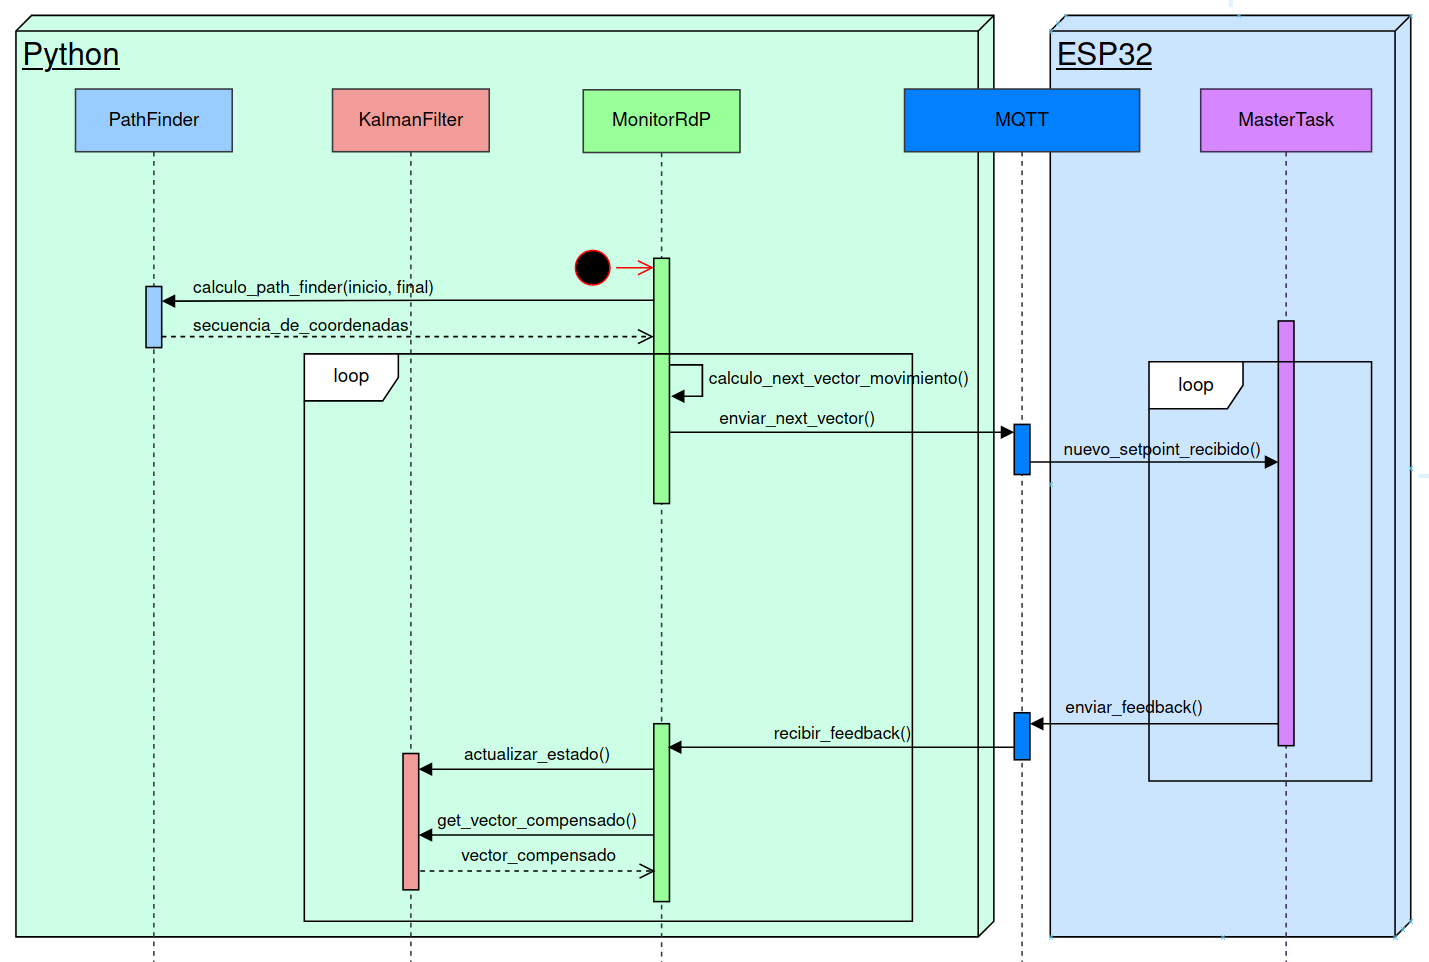
\includegraphics[width=1.15\linewidth]{images/diag_secuencia_filtro_de_kalman_con_esp32.png}
    \caption{Diagrama de secuencia con el Filtro de Kalman}
    \label{fig:diagsecuenciafiltrokalman}
\end{figure}


\textbf{Modelo del filtro} \mbox{} \vspace{10pt}

El filtro de Kalman requiere que modelemos matemáticamente nuestro sistema. En nuestro caso registraremos la posición y velocidad en un eje determinado. El modelo matemático es en base a la ecuación de movimiento rectilíneo acelerado, por lo que para la posición y velocidad instantáneas se tiene:

$$ x = x_0 + x_0 \Delta t + \frac{1}{2} a \Delta t^2 $$
$$ v_x = v_0 + a\Delta t $$

\textbf{Cálculo del Estado Predicho $X_{kp}$} \mbox{} \vspace{10pt}

Este término significa en donde debería estar el robot según el modelo ideal y la distancia entre muestras $\Delta t$. En base a lo anterior en forma matricial, tenemos que el estado predicho está dado por:

$$ X_{kp} =
    \begin{bmatrix} x_{kp} \\ v_{kp} \\ \end{bmatrix}
    =
    A \cdot X_{k-1} + B \cdot U_k + \omega_k
$$

Las matrices A y B representan al modelo en base a las ecuaciones de arriba, mientras que $\omega_k$ representa algún ruido o perturbación presente en el proceso de cálculo del estado predicho. En nuestro caso lo consideramos despreciable, por lo que es nulo. Además, el vector $U_k$ se considera nulo dado que no llevaremos registro de la aceleración del robot.

Donde:

$$
X_{k-1} = \begin{bmatrix} x_{k-1} \\ v_{k-1} \\ \end{bmatrix}
;
A = \begin{bmatrix}
    1 & \Delta t  \\
    0 & 1         \\
    \end{bmatrix} \\
;
B = \begin{bmatrix}
    \frac{1}{2} \Delta t^2 \\
    \Delta t               \\
    \end{bmatrix}          \\
;
U_k = \begin{bmatrix} a_0 \\ \end{bmatrix} \\
;
\omega_k = \begin{bmatrix} 0 \\ 0 \\ \end{bmatrix}
$$

Entonces la ecuación para obtener el nuevo estado predicho:

$$
X_{kp} = 
    \begin{bmatrix}
    1 & \Delta t  \\
    0 & 1         \\
    \end{bmatrix} \\
    \cdot \begin{bmatrix} x_{k-1} \\ v_{k-1} \\ \end{bmatrix}
    +
    \begin{bmatrix}
    \frac{1}{2} \Delta t^2 \\
    \Delta t               \\
    \end{bmatrix}          \\
    \cdot
    \begin{bmatrix} 0 \\ \end{bmatrix} \\
    +
    \begin{bmatrix} 0 \\ 0 \\ \end{bmatrix}
$$ \\

\textbf{Cálculo de Matriz de Covarianza de Proceso Predicha $P_{kp}$} \mbox{} \vspace{10pt}

Esta matriz se modela teniendo por un lado el término $\Delta_{px}$ y por otro lado el término $\Delta_{pv_x}$ que representan errores en el proceso de calcular la posición y velocidad predichos.

En el caso que exista relación en la incerteza del proceso para calcular la posición y velocidad, el término $\Delta_{px} \cdot \Delta_{pv_x}$ es distinto de cero. En nuestro caso lo establecemos en $0$.

Por lo que se tiene la siguiente matriz de covarianza inicial:

$$
P_{k-1} = \begin{bmatrix}
    {\Delta_{px}}^2 & \Delta_{px} \cdot \Delta_{pv_x} \\
    \Delta_{px} \cdot \Delta_{pv_x} & {\Delta_{pv_x}}^2 \\
    \end{bmatrix} \\
    = \begin{bmatrix}
    {\Delta_{px}}^2 & 0 \\
    0 & {\Delta_{pv_x}}^2 \\
    \end{bmatrix} 
$$

Luego, para calcular la nueva matriz se parte de la siguiente expresión:

$$ P_{kp} = A \cdot P_{k-1} A^T + Q_k $$

Donde la matriz A es la misma expresada en el paso anterior y $Q_k$ modela el error en el proceso de cálculo de las matrices de covarianza, también establecido en $0$. Por lo que obtenemos:

$$ P_{kp} =
    \begin{bmatrix}
    1 & \Delta t  \\
    0 & 1         \\
    \end{bmatrix} \\
    \cdot 
    \begin{bmatrix}
    {\Delta_{px}}^2 & 0   \\
    0 & {\Delta_{pv_x}}^2 \\
    \end{bmatrix}
    \cdot
    \begin{bmatrix}
    1 & 0           \\
    \Delta t & 1    \\
    \end{bmatrix}   \\
    +
    \begin{bmatrix}
    0 & 0  \\
    0 & 0  \\
    \end{bmatrix}  \\
$$

\textbf{Cálculo de la ganancia de Kalman $K$} \mbox{} \vspace{10pt}

La ganancia de Kalman en pocas palabras es una media ponderada que le da mas o menos importancia a la medición versus la estimación según el error detectado. Si la ganancia $K$ tiende a 0, indica que el sistema no converge y que tiene un error considerable. Por otro lado si la ganancia $K$ tiende a 1 indica que tiene poco error.

Para calcular la ganancia de Kalman utilizamos la siguiente expresión:

$$ K = \frac{P_{kp} \cdot H^T}
            {H \cdot P_{kp} \cdot H^T + R}
$$

Donde la matriz $H$ es una matriz identidad $I$ que se utiliza para convertir el dominio de los datos al formato que necesita $K$. La matriz $R$ es una matriz de covarianzas que representa los errores en la observación, que se puede simplificar del mismo modo que $P_{kp}$ y se puede expresar como:

 $$ R =
    \begin{bmatrix}
    {\Delta_x}^2 & \Delta_x \cdot \Delta_{v_x} \\
    \Delta_x \cdot \Delta_{v_x} & {\Delta_{v_x}}^2 \\
    \end{bmatrix} \\ 
    =
    \begin{bmatrix}
    {\Delta_x}^2 & 0 \\
    0 & {\Delta_{v_x}}^2 \\
    \end{bmatrix} \\ 
$$

Por lo que para calcular la ganancia de Kalman:

$$ K =
    \frac{
        \begin{bmatrix}
        {\Delta_{px}}^2 & 0 \\
        0 & {\Delta_{pv_x}}^2 \\
        \end{bmatrix}
        \cdot
        \begin{bmatrix}
        1 & 0 \\
        0 & 1  \\
        \end{bmatrix}
        }
    {
        \begin{bmatrix}
        1 & 0 \\
        0 & 1  \\
        \end{bmatrix}
        \cdot
        \begin{bmatrix}
        {\Delta_{px}}^2 & 0 \\
        0 & {\Delta_{pv_x}}^2 \\
        \end{bmatrix}
        \cdot
        \begin{bmatrix}
        1 & 0 \\
        0 & 1  \\
        \end{bmatrix}
        +
        \begin{bmatrix}
        {\Delta_x}^2 & 0 \\
        0 & {\Delta_{v_x}}^2 \\
        \end{bmatrix} \\ 
    }
$$ \\

\textbf{Cálculo del Estado Estimado $X_k$} \mbox{} \vspace{10pt}

Para obtener la nueva estimación del estado en base a la última medición recibida, podemos expresar:

$$ X_k = X_{kp} + K \cdot ( Y_k - H \cdot X_{kp} ) $$

Donde $X_{kp}$ es el estado predecido, $K$ es la ganancia de Kalman, $Y_k$ es la medición observada y $H$ una matriz de conversión. Esta ultima resulta ser una matriz identidad por no ser necesario convertir los datos del estado predicho.

$$ X_k =
    X_{kp}
    +
    K
    \cdot (
        \begin{bmatrix} x_{km} \\ v_{km} \\ \end{bmatrix}
        -
        \begin{bmatrix}
        1 & 0 \\
        0 & 1  \\
        \end{bmatrix}
        \cdot
        X_{kp}
    )
$$ \\

\textbf{Actualización de la Matriz de Covarianza de Proceso $P_k$} \mbox{} \vspace{10pt}

Eventualmente, cuando el error se reduce lo suficiente, podemos actualizar la matriz de covarianza de proceso mediante la siguiente expresión:

$$ P_k = ( I - K \cdot H ) \cdot P_{kp} $$

Donde $H$ nuevamente es una matriz identidad. Por lo que resulta:

$$ P_k =
    (
    \begin{bmatrix}
    1 & 0 \\
    0 & 1  \\
    \end{bmatrix}
    -
    K
    \cdot
    \begin{bmatrix}
    1 & 0 \\
    0 & 1  \\
    \end{bmatrix}
    )
    \cdot
    P_{kp}
$$

\textbf{Actualización de valores} \mbox{} \vspace{10pt}

Antes de comenzar una nueva iteración debemos actualizar los valores de la matriz de covarianza y la de estado predecido:

$$ P_{k-1} = P_k $$
$$ X_{k-1} = X_k $$